%%%%%%%%%%%%%%%%%%%%%%%%%%%%%%%%%%%%%%%%%
% Masters/Doctoral Thesis 
% LaTeX Template
% Version 1.41 (9/9/13)
%
% This template has been downloaded from:
% http://www.latextemplates.com
%
% Original authors:
% Steven Gunn 
% http://users.ecs.soton.ac.uk/srg/softwaretools/document/templates/
% and
% Sunil Patel
% http://www.sunilpatel.co.uk/thesis-template/
%
% License:
% CC BY-NC-SA 3.0 (http://creativecommons.org/licenses/by-nc-sa/3.0/)
%
% Note:
% Make sure to edit document variables in the Thesis.cls file
%
%%%%%%%%%%%%%%%%%%%%%%%%%%%%%%%%%%%%%%%%%

%----------------------------------------------------------------------------------------
%	PACKAGES AND OTHER DOCUMENT CONFIGURATIONS
%----------------------------------------------------------------------------------------

\documentclass[11pt, a4paper, oneside]{Thesis} % Paper size, default font size and one-sided paper

\graphicspath{{Pictures/}} % Specifies the directory where pictures are stored

\usepackage[square, numbers, comma, sort&compress]{natbib} % Use the natbib reference package - read up on this to edit the reference style; if you want text (e.g. Smith et al., 2012) for the in-text references (instead of numbers), remove 'numbers' 
\hypersetup{urlcolor=blue, colorlinks=true} % Colors hyperlinks in blue - change to black if annoying
\title{\ttitle} % Defines the thesis title - don't touch this

\begin{document}

\frontmatter % Use roman page numbering style (i, ii, iii, iv...) for the pre-content pages

\setstretch{1.3} % Line spacing of 1.3

% Define the page headers using the FancyHdr package and set up for one-sided printing
\fancyhead{} % Clears all page headers and footers
\rhead{\thepage} % Sets the right side header to show the page number
\lhead{} % Clears the left side page header

\pagestyle{fancy} % Finally, use the "fancy" page style to implement the FancyHdr headers

\newcommand{\HRule}{\rule{\linewidth}{0.5mm}} % New command to make the lines in the title page

% PDF meta-data
\hypersetup{pdftitle={\ttitle}}
\hypersetup{pdfsubject=\subjectname}
\hypersetup{pdfauthor=\authornames}
\hypersetup{pdfkeywords=\keywordnames}

%----------------------------------------------------------------------------------------
%	TITLE PAGE
%----------------------------------------------------------------------------------------

\begin{titlepage}
\begin{center}

\textsc{\LARGE \univname}\\[1.5cm] % University name
\textsc{\Large Doctoral Thesis}\\[0.5cm] % Thesis type

\HRule \\[0.4cm] % Horizontal line
{\huge \bfseries \ttitle}\\[0.4cm] % Thesis title
\HRule \\[1.5cm] % Horizontal line
 
\begin{minipage}{0.4\textwidth}
\begin{flushleft} \large
\emph{Author:}\\
\href{http://www.johnsmith.com}{\authornames} % Author name - remove the \href bracket to remove the link
\end{flushleft}
\end{minipage}
\begin{minipage}{0.4\textwidth}
\begin{flushright} \large
\emph{Supervisor:} \\
\href{http://www.jamessmith.com}{\supname} % Supervisor name - remove the \href bracket to remove the link  
\end{flushright}
\end{minipage}\\[3cm]
 
\large \textit{A thesis submitted in fulfilment of the requirements\\ for the degree of \degreename}\\[0.3cm] % University requirement text
\textit{in the}\\[0.4cm]
\groupname\\\deptname\\[2cm] % Research group name and department name
 
{\large \today}\\[4cm] % Date
%\includegraphics{Logo} % University/department logo - uncomment to place it
 
\vfill
\end{center}

\end{titlepage}




%----------------------------------------------------------------------------------------
%	LIST OF CONTENTS/FIGURES/TABLES PAGES
%----------------------------------------------------------------------------------------

\pagestyle{fancy} % The page style headers have been "empty" all this time, now use the "fancy" headers as defined before to bring them back

\lhead{\emph{Contents}} % Set the left side page header to "Contents"
\tableofcontents % Write out the Table of Contents

\lhead{\emph{List of Figures}} % Set the left side page header to "List of Figures"
\listoffigures % Write out the List of Figures

\lhead{\emph{List of Tables}} % Set the left side page header to "List of Tables"
\listoftables % Write out the List of Tables



%----------------------------------------------------------------------------------------
%	THESIS CONTENT - CHAPTERS
%----------------------------------------------------------------------------------------

\mainmatter % Begin numeric (1,2,3...) page numbering

\pagestyle{fancy} % Return the page headers back to the "fancy" style

% Include the chapters of the thesis as separate files from the Chapters folder
% Uncomment the lines as you write the chapters

% Chapter 1

\chapter{Introduction} % Main chapter title

\label{Chapter1} % For referencing the chapter elsewhere, use \ref{Chapter1} 

\lhead{Chapter 1. \emph{Introduction}} % This is for the header on each page - perhaps a shortened title

%----------------------------------------------------------------------------------------
Every person in his life at least once leaves his home city for any reason, whether it is a business trip or just a vacation. Taking into account that modern technologies nowadays allow people to move from one point to another in a few hours, such trips becomes much easier to perform. Moreover it gives an opportunity to investigate almost every point on the globe. 

That is why maps become indispensable attribute of any trip. There are two main categories of maps: paper and electronic maps. Classical paper maps can help in any situation but in comparison with electronic map they have one big disadvantage – they are not interactive. Electronic maps in its turn are also separated on "online" and "offline" maps. "Online" maps are interactive, fast and usually not limited to one city. Furthermore there is more than one "online" map, so user can use any on his taste. 

But what to do if for any reason there is no internet connection? For this case "offline" maps can be used, especially if person appears in unknown city. And the main problem of any map that covers large area in this case can be absence of any important information like presence of grocery store or bakery or laundry for small cities. That is why implementation of maps for small areas and cities is very important, because it contains specific information about this particular region.

So the goal of our project was implementation of the map for city Le Creusot with basic set of data and functions like finding way between two points or showing main public facilities. It can be useful for any person whether it's a tourist, visitor on a business trip or a student. Especially we hope that this map can be useful for next \textit{ViBOT/MsCV} promotions for simplifying their life in Le Creusot.

% Chapter 2

\chapter{Project management} % Main chapter title

\label{Chapter2} % For referencing the chapter elsewhere, use \ref{Chapter1} 

\lhead{Chapter 2. \emph{Project management}} % This is for the header on each page - perhaps a shortened title

%----------------------------------------------------------------------------------------
In this chapter we want to present how our group organized and managed this project. Group members are:
\begin{itemize}
\item Oksana Hagen
\item Natalia Shepeleva
\item Emre Ozan Alkan
\item Klemen Istenič
\end{itemize}
As we all had a bit of experiences in software design, we knew how important a proper plan and research before the actual implementation is. Unfortunately, we were also aware that no matter how good the plan is, we will be forced to adjust it during the implementation. Either because of the things we overlooked while planning or because some assumptions we made were wrong. We decided to follow the \textit{iterative and incremental development model}, which enabled us to adjust our plans after each of the implementation iterations. A schematic representation of the iterative and incremental development model can be seen on figure \ref{fig:Iterative_development_model_V2}.
\begin{figure}[h]
\centering
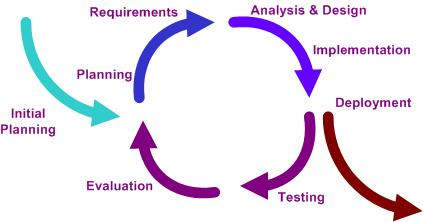
\includegraphics[height=4cm]{../pictures/Iterative_development_model_V2}
\caption{An iterative development model (image taken from \cite{wiki1})}
\label{fig:Iterative_development_model_V2}
\end{figure}

\section{Basic building blocks}
\label{Building blocks}
On our first meeting we decided to split the project into four main parts to be able to fully manage the whole project at all times. This parts are:
\begin{itemize}
\item User interface
\item Database and data structure
\item Map representation
\item Path algorithms
\end{itemize}

\subsection{UI - User Interface}
Part of the application that is responsible for user interaction with the application. Main goal is to make the interface as user-friendly as possible. In the beginning we made a rough sketch of how the interface should look (figure \ref{fig:sketch}), which has, as expected, changed during the process of later design and implementation. The UI is presented more in details in chapter [UI USER MAUNAL].
\begin{figure}[h]
\centering
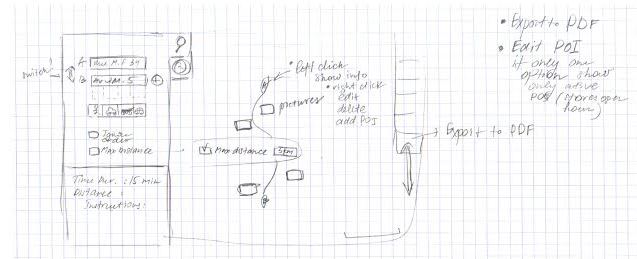
\includegraphics[width=0.6\linewidth]{../pictures/sketch.jpg}
\caption{Inital sketch of UI}
\label{fig:sketch}
\end{figure}
\subsection{Database and data structure}
Our database consists of two parts. The static part, having the information about the roads in Le Creusot (described in []) and the dynamic part with the information about the points of interest (POI). In chapter[] we address the facts we took into account while considering different database options and data structures.
\subsection{Map representation}
We separated map representation from other parts of user interface, because we think it is the most important of UI, so we will give special attention to it.
\subsection{Path algorithms}
In the different algorithms we adopted and developed, we do all the searching for paths, calculating distance and travel times and optimize the search results as much as possible. Our main goal is to make the algorithms work as  quickly as possible, taking into account all the restrictions road networks has (one way streets, foot ways etc.). We also want to make the algorithms as reusable as possible, to reduce the redundancy in development and minimize the possibilities of errors.


\section{Meetings and Project Progress}

Development stages can be divided in three parts. First stage included analyzing the problem, extracting project requirements and devising a plan for the implementation. Second part included extracting the application structure, collecting most appropriate tools for the implementation and setting up the environment. The last part is the implementation itself starting from building the basic blocks, simple prototype application and then gradually adding functionalities and features, along wise with documenting the software. All the stages were supported with meetings according to time constraints and project progress speed.

\subsection{Analyzing the problem}
Fist meetings were devoted to the analyzing the provided requirements and inventing all possible useful features. Besides the general idea of user interface was developed according to all the needed functionality of the project. The scope of the project was defined and future work planned.

\subsection{Pre-implementation stage}
In the later meetings we were considering architecture challenges and possible solutions, able to provide the need functionality for the application. We were focusing on extracting the most appropriate tools and libraries to ease the development process as well as getting the idea . After it was done the same development environment was set up on all the computers. At this point it was clear how the implementation will differ in Matlab and C++ and the team got slitted between Matlab and C++ development.

\subsection{Implementation}
All next meetings were devoted to the coding the application and solving particular issues. At this stage separate basic blocks (ui, map-rendering, database, algorithms) were developed and then merged in one working application prototype, which only consisted of two-point path search. When it was clear that all the framework decisions were reasonable, further development was done.

\section{Software used for project management}
At first and second stage Dropbox was used to share latest meeting reports, schematics, useful papers and links. On the last stage the need of tool for simultaneous development became obvious. For that purpose, we chose GitHub repository hosting service. Besides, it was extremely useful for tracking issues and bugs. At very last meetings we used Skype conferences, since all the project team members were in different places.
 
% Chapter 2

\chapter{Initial planning} % Main chapter title

\label{Chapter3} % For referencing the chapter elsewhere, use \ref{Chapter1} 

\lhead{Chapter 3. \emph{Initial planning}} % This is for the header on each page - perhaps a shortened title

%----------------------------------------------------------------------------------------
\section{User requirement analysis}
\label{(user_req)}
As mentioned in the previous chapter, we decided to use \textit{the iterative and incremental development model}. Before starting the iterations we spend quite a lot of time on the initial planning, with special attention to user and general project requirement analysis. From the project's instructions we were able to identify the following major user requirements and construct use case diagram (figure \ref{fig:gen_use_case_diag}):
\begin{itemize}
\item User should be able to enter start and end point either by:
\begin{itemize}
\item mouse click;
\item specifying latitude and longitude;
\item selecting a point of interest.
\end{itemize}
\item Find shortest path from point A to B (by foot or by car);
\item Find the shortest way to all POIs of a certain category in a radius from point A (by foot or by car);
\item Construct an itinerary from point A to B with visiting POIs in between (with max distance limit);
\item View, edit and add POIs
\end{itemize}

\begin{figure}[h]
\centering
\includegraphics[width=0.95\linewidth]{../pictures/use_case_diagram_general}
\caption{Use case diagram}
\label{fig:gen_use_case_diag}
\end{figure}

\section{Plan of implementation}
After having the user requirements, we decided to make the global plan of implementation. We took into account the fact that we have to develop the applications in \textbf{C++} and \textbf{Matlab}. As described in section \ref{Building blocks}, we have already split the project into four main parts. Because the user interface and map representations require completely different approaches in C++ and Matlab, we decided to split them into two parallel projects, one almost independent from another. On the other hand, we decided to use the same algorithms for both projects. The main reason is the minimization of the redundancies in the research and development stage and reducing the possibility of errors. This way we could have the same algorithms for both, differing only in pure implementation details.



% Chapter 2

\chapter{Data sources} % Main chapter title

\label{Chapter4} % For referencing the chapter elsewhere, use \ref{Chapter1} 

\lhead{Chapter 4. \emph{Data sources}} % This is for the header on each page - perhaps a shortened title

%----------------------------------------------------------------------------------------
Our application uses two main types of data. \textbf{Static} map data describing the streets and buildings and \textbf{dynamic} data about the different points of interest (POIs). The difference between static and dynamic data lies in the users ability to add and edit POI, while the map information is not meant to be changed by the user.
\par The acquisition of this data was not the essence of the project, so we were allowed to use any data source, with appropriate licence and collaborate with other groups. 

\section{Map data - OpenStreetMap}
Acquisition of map data (roads, road types, buildings etc.) can be extremely time consuming and can easily produce unreliable results. At the same time, there are a lot of different open source data sources available on-line. Together with the other groups we decided to use OpenStreetMap data by the OpenStreetMap Foundation (\cite{osm}).
\par OpenStreetMap is an open source project providing free map data of the world. Data is published under the \textit{Open Database License (ODbL) from Open Data Commons (ODC)}, which enables us to freely produce the works from the database, modify, transform and build upon the database.

\subsection{Data format}
OpenStreetMap data consists of four core elements:
\begin{itemize}
\item \textbf{Nodes} - basic point of location with longitude and latitude information. They can be used to mark a single point (POI) or in a list of nodes (way, relation);
\item \textbf{Ways} - ordered list of nodes, representing a street or an area like a lake, forest etc.;
\item \textbf{Relations} - ordered list of nodes and ways which can be in a relation (many different roads can be part of a long motorway);
\item \textbf{Tags} - key-value pairs which are used to store information about different objects (nodes, ways, relations).
\end{itemize}
Figure \ref{fig:Osm_flow} shows the difference between different core elements
\begin{figure}[h]
\centering
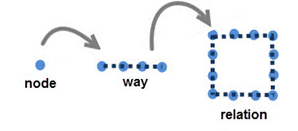
\includegraphics{../pictures/osm_flow.png}
\caption{Representation of basic OSM elements (image taken from \cite{osm_2})}
\label{fig:Osm_flow}
\end{figure}

\section{Points of Interest (POI)}
One of the main requirements for our application is to enable user to search using different points of interest. For acquisition of this points, all of the groups again collaborated, each marking all the points in one part of Le Creusot. For each point we decided to acquire:
\begin{itemize}
\item name;
\item location;
\item address;
\item photo.
\end{itemize}
In the end we also categorized all the points into 26 different categories. 
 
% Chapter 2

\chapter{Database and data structure} % Main chapter title

\label{Chapter5} % For referencing the chapter elsewhere, use \ref{Chapter1} 

\lhead{Chapter 5. \emph{Database and data structure}} % This is for the header on each page - perhaps a shortened title

%----------------------------------------------------------------------------------------

\section{Database}
As described, our data consists of two parts. \textit{Static} map data and \textit{dynamic} points of interests data. For the beginning, we were deciding between using relational database and XML based database. With each of them having some benefits, we took the following facts intro account during the consideration:
\begin{itemize}
\item Most of the data is static - information about the roads in Le Creusot will not change;
\item Dynamic data will rarely change - user will not often update information about the points of interest;
\item Relatively small amount of data - Le Creusot is a small city, so there is not a lot of information about the roads. This gives us the opportunity to read all the information to memory at the beginning, reducing the latency caused by queries to the database;
\item Easiness of install and mobility -  using relational database, requires installation of different software (SQL server, connectors, etc.) on the clients computer, which we wanted to avoid. 
\end{itemize} 
In the end we decided to use \textbf{XML based database}. We kept the two parts of the data split into separate XML files. We kept the OpenStreetMap data in the OSM file and created another XML file for POI data. This way, we could easily change either part of the data without compromising the other.
\subsection{Disadvantage}
Using XML based database has one big disadvantage, which we have to take into account. XML based database is saved into a file. This does not provide the ability to easily update POI data. Unfortunately, every time we update this data, we have to rewrite the whole file. This can in some occasions be the source of problems, as the writing to the file can be disrupted or cancelled, making the file unusable. However, we do not anticipate the user to update the data frequently, so we took this compromise.

\section{Data structure}
We have designed out class structure with the A* search algorithm and OpenStreetMap (OSM) file structure in mind. We followed the OSM structure, having a basic class called \textbf{Node}. In figure \ref{fig:types_db} we show the different types of classes we use with a small graphic representation for better understanding.
\begin{figure}[h]
\centering
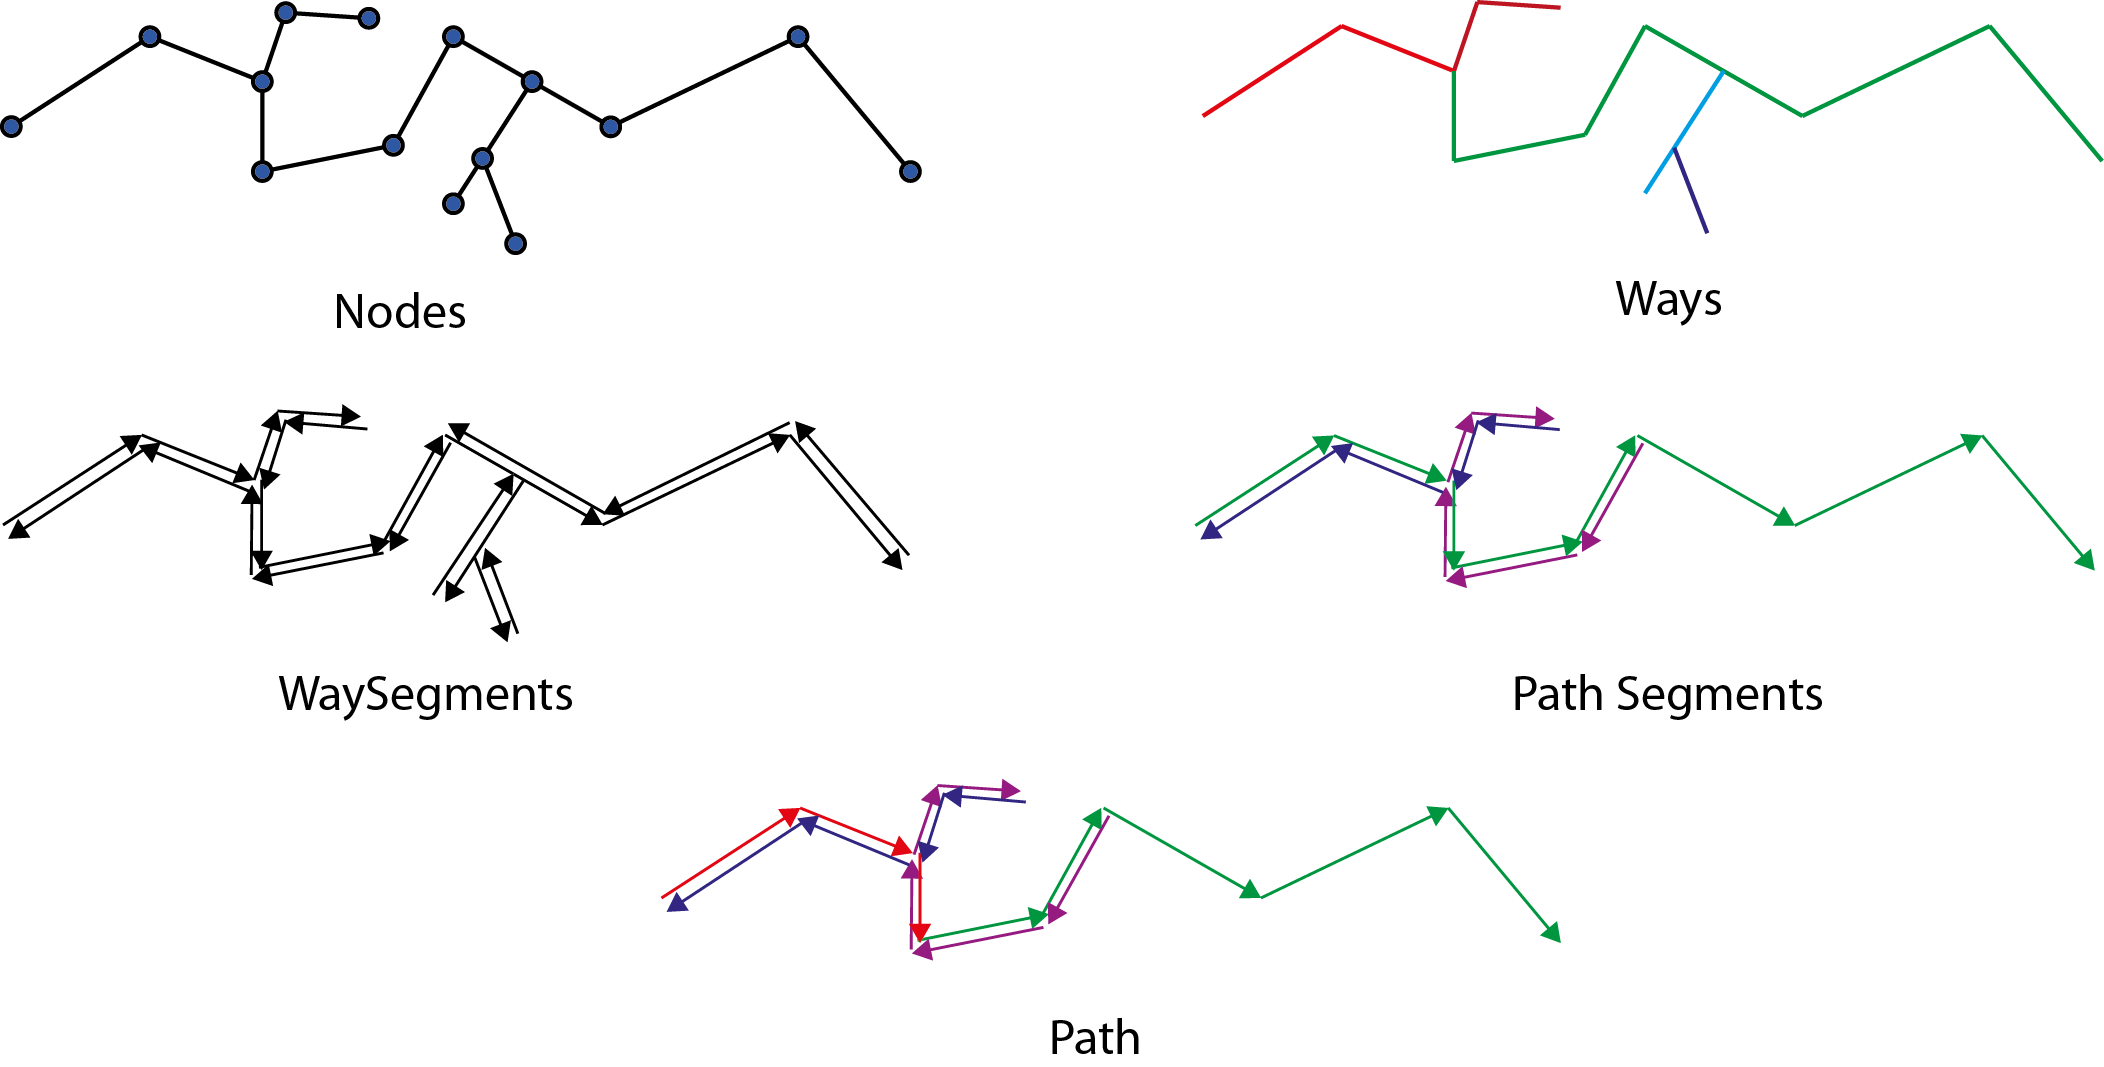
\includegraphics[width=0.8\linewidth]{../pictures/ways.png}
\caption{Different objects in our data structure}
\label{fig:types_db}
\end{figure}
\subsubsection{Node class}
It is used to represent a single point on the map. This can either mark a point of interest (POI), or can be a part of a Relation such as \textit{WaySegment, Building or Way}. It contains location information, some A* algorithm informations (weights, visited flags, etc.) and a vector of pointers of WaySegments to which we can traverse from this Node. This is important especially for A* algorithm, as it significantly reduce the time needed to find all possible and subsequently the correct next move.

\subsubsection{Way class}
Class implemented as in OSM file, to store the properties of each of the ways. It us usually used to represent whole streets, or part of the street that have the same properties. Each way is assigned a type (primary, secondary, etc.), direction (one-way, bidirectional) and access privileges (private or public).

\subsubsection{Relation class}
Relation is a base class from which we extend different relation classes (WaySegment, Building). It only contains a vector of pointers to Nodes that are in one specific relation and type of the relation.

\subsubsection{WaySegment class}
WaySegment is the main class for our path algorithms. WaySegment connects two nodes in a specific direction. This means that if the road between two nodes is bidirectional, we will create two WaySegment objects, one for each direction. We also have a pointer to an object Way, which belongs to the road traversing. This gives us the option of getting information about the road at any time.

\subsubsection{Building class}
Is a simple class containing all the nodes representing one building.

\subsubsection{PathSegment class}
It is a class that is used to store the result of a \textit{shortest path search}. It contains all the pointers to WaySegment objects we need to traverse in order to get from point A to B. 

\subsubsection{Path class}
Object that contains vector of PathSegment pointers. Path is the end result of any search. If the search is solely path from point A to B, the path is going to have only one PathSegment pointer. On the other hand, if we search for itinerary, Path will include multiple PathSegments, one for each pair of middle points.

\subsubsection{Database class}

Database is an main class for the whole database. It contains functions for correct parsing of XML files and also has containers \textit{(std::map)} with pointers to each of the classes created (Node,Way,Bulding,WaySegment). We use this to quickly retrieve the classes based on their ID, and to be sure to delete all created objects in the destructor of the class. We also used a boost implementation of a \textit{rtree} data structure to hold all the WaySegment objects to be able quickly do a spatial filtering. This is very useful in implementation of finding the close WaySegments.
\par
In figure \ref{fig:db_class} we can see the whole class diagram of the database part of the application in C++.
 \begin{figure}[h]
 \centering
 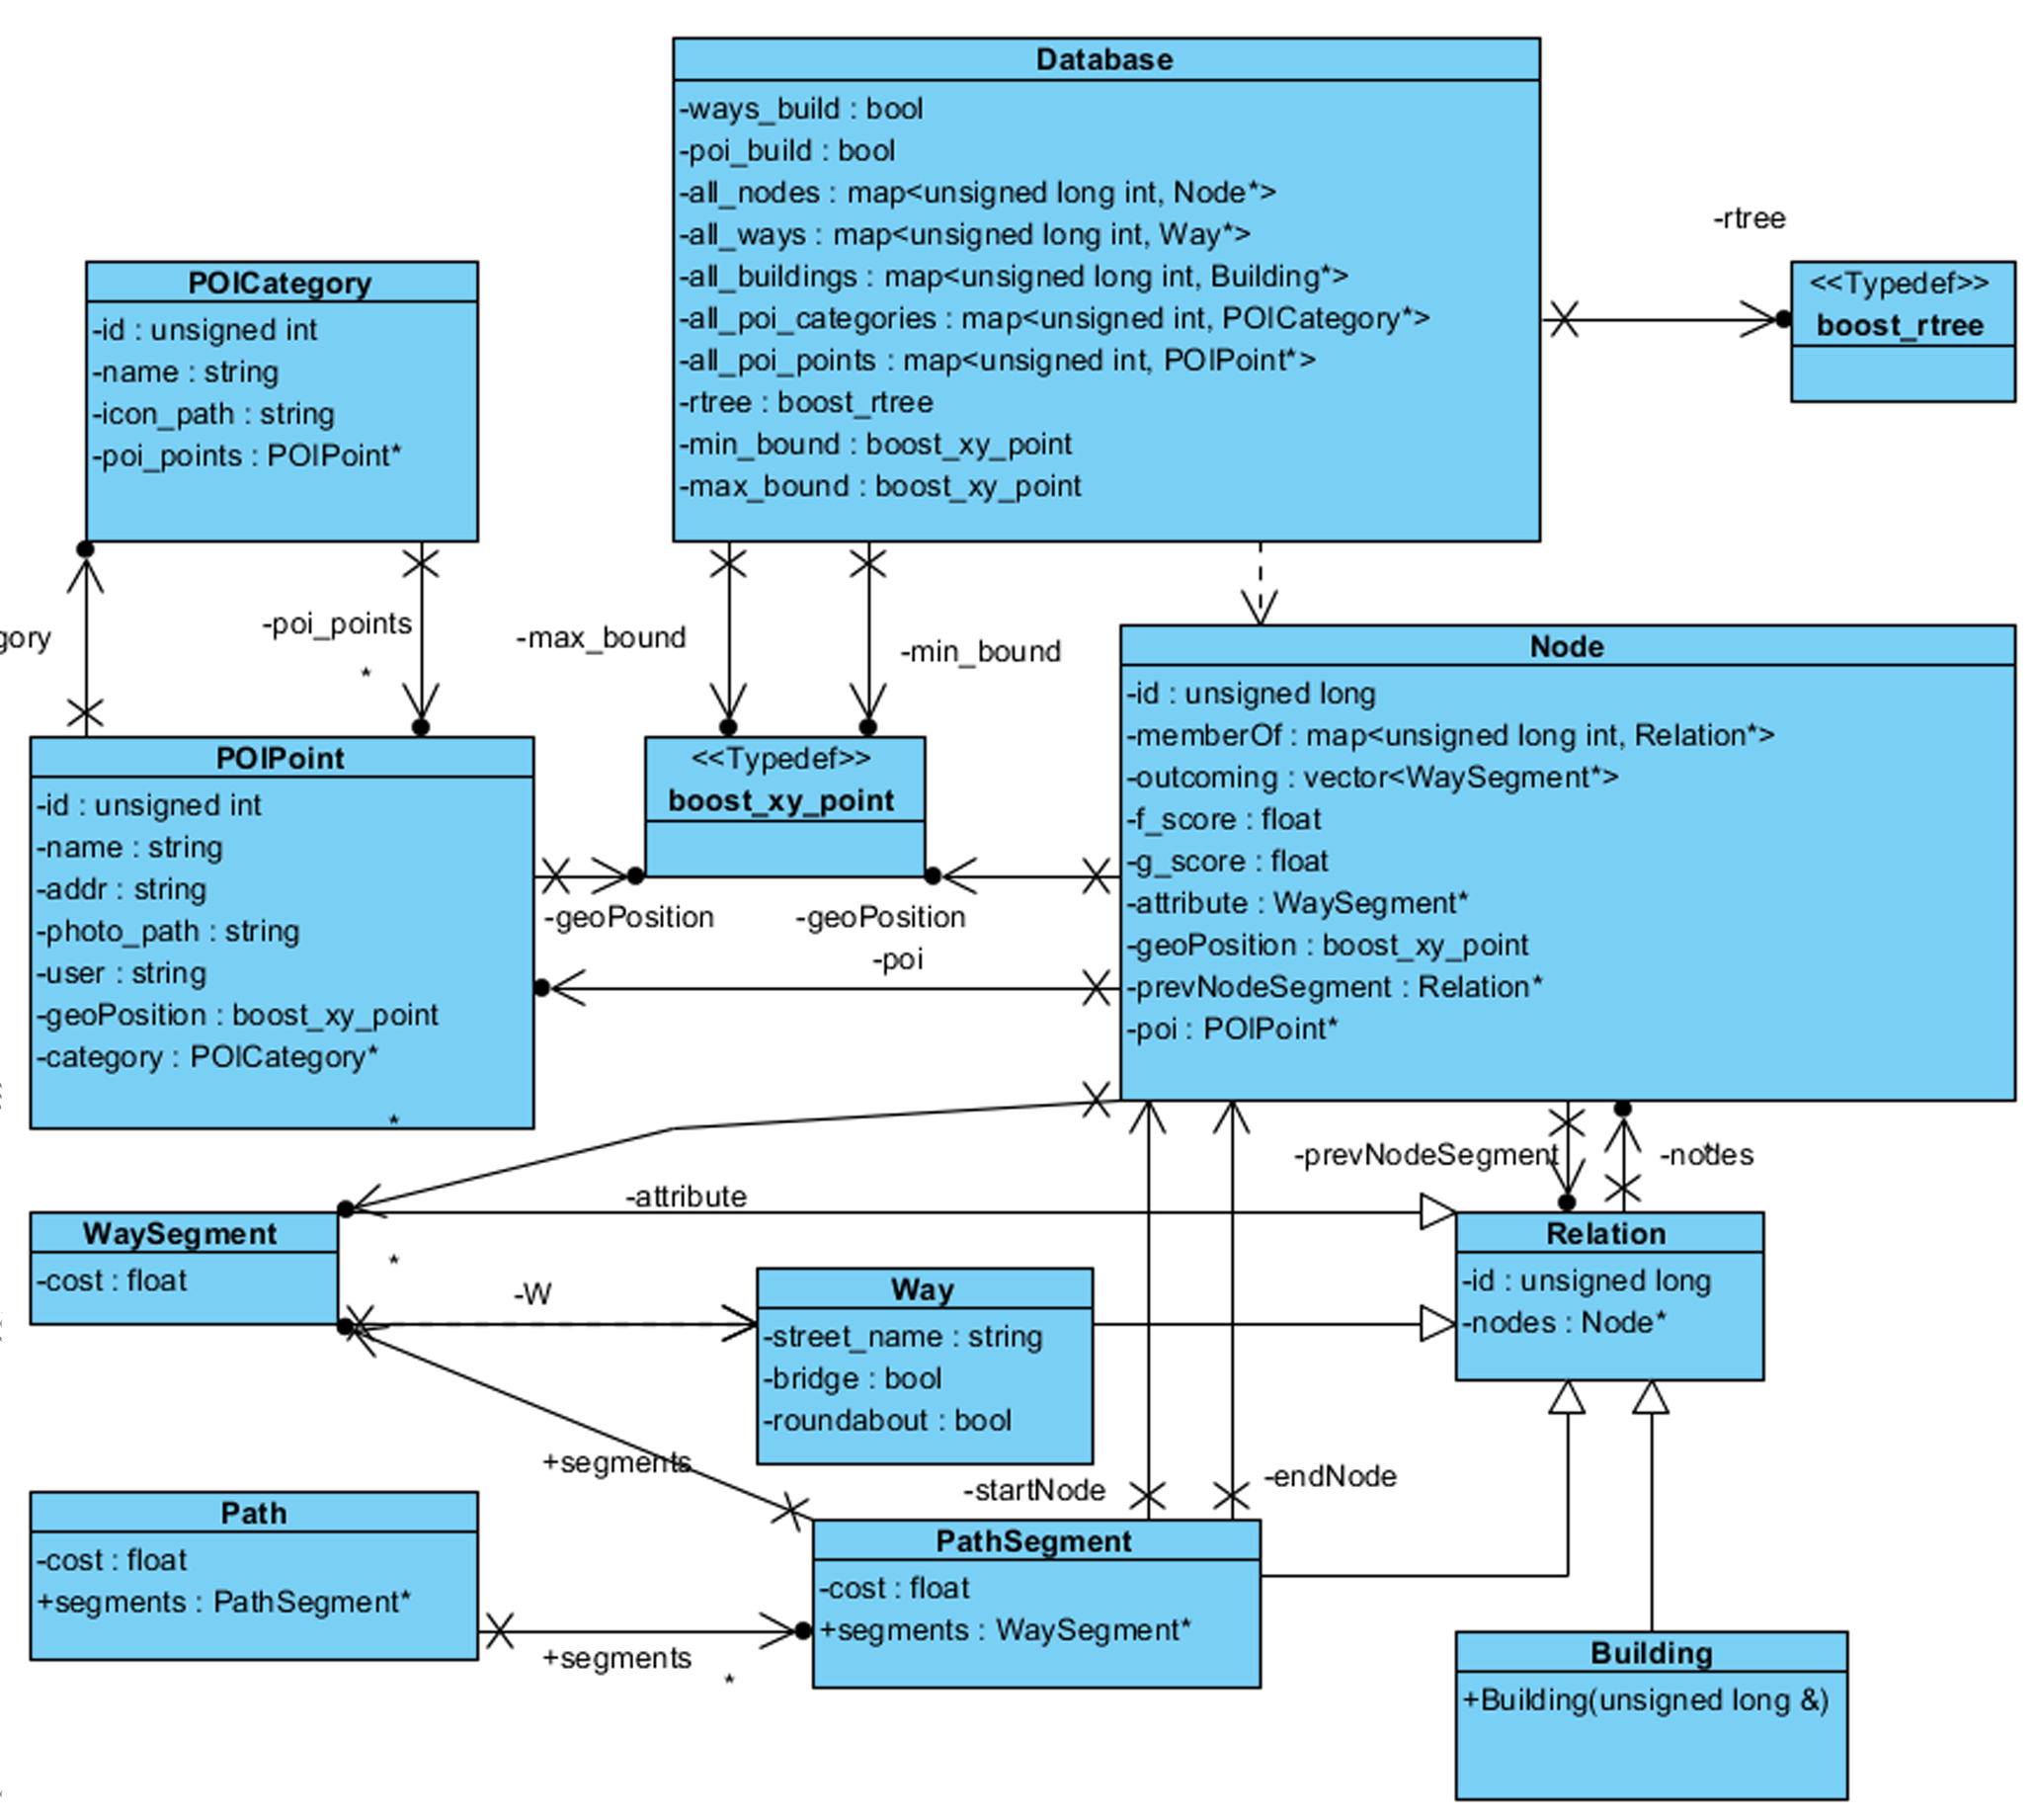
\includegraphics[width=0.9\linewidth]{../pictures/Class_Diagram.png}
 \caption{Class diagram}
 \label{fig:db_class}
 \end{figure}

 
%% Chapter 2

\chapter{Path algorithms} % Main chapter title

\label{Chapter6} % For referencing the chapter elsewhere, use \ref{Chapter1} 

\lhead{Chapter 6. \emph{Path algorithms}} % This is for the header on each page - perhaps a shortened title

%----------------------------------------------------------------------------------------
Finding the shortest path is one of the main problems in graph theory. It is a problem of finding a path between two nodes, where the sum of edge weights must be minimized. Graph can be undirected, directed or mixed.
\par The analogy with road maps can be clearly seen, where nodes correspond to intersections and road segments to edges on the graph. To properly represent one way streets we use directed graph. The weight of each edge can be interpreted as a length of each road segment.
\par There are numerous algorithms that are able to found the shortest path. After initial research we narrowed the possible algorithms to:
\begin{itemize}
\item Dijkstra's algorithm
\item A* search algorithm
\item Bellman - Ford algorithm
\item Floyd - Warshall algorithm
\end{itemize}
From the user requirement analysis (segment \ref{user_req}) we were able to identify the three main user requests involving path algorithms:
\begin{itemize}
\item Find shortest path from point A to B (by foot or by car);
\item Find the shortest way to all POIs of a certain category in a radius from point A (by foot or by car);
\item Construct an itinerary from point A to B with visiting POIs in between (with max distance limit);
\end{itemize}

From identified requirements, we can see that all of our path finding problems are actually problems of finding paths between points A and B. This are so-called \textbf{single-pair shortest path problems}. Analysing the algorithms listed above we determined that:
\begin{itemize}
\item Floyd - Warshall algorithm finds shortest paths between every pair of nodes in the graph;
\item Dijkstra and Bellman - Ford algorithms find the shortest paths between source node and all other nodes on the graph (Bellman - Ford also permits negative weights);
\item A* algorithm finds the shortest path between the source and target node. 
\end{itemize}

All of the above algorithms encapsulate the result which we need, but differing in how many unnecessary paths are also calculated. This subsequently mean longer calculation times, which we want to avoid. For this reasons we chose \textbf{A* algorithm} for our path finding problems.

\section{A* algorithm}
A* algorithm is one of the most popular path finding algorithms. Its ability to combine the benefits of Dijkstra's algorithm (favouring nodes close to the start node) and Best-First-Search algorithms (favouring nodes close to the target node) makes it efficient and accurate. 
\subsection{Process}
Algorithm works by traversing the graph node by node till it reaches the end node. At every step, node with the lowest cost $(f(x))$ is selected. Calculation of the cost and selection of the node is what sets A* algorithm apart from other greedy best-first search algorithms. Cost is calculated as a weighted sum of:
\begin{itemize}
\item $g(n) - $\textit{exact cost} of the path from the starting point,
\item $h(n) - $\textit{heuristic estimated cost}.
\end{itemize}
Heuristics are used to control the A*'s behaviour. If $h(n)=0$ only distance from the start node matters and we have normal Dijkstra algorithm. Because we do not know the real distance from observed node to the end target, as we haven't traversed it yet, we have to estimate it. It is important not to overestimate the distance, as this can cause the algorithm not to found the shortest path. We decided to use the air distance as a heuristic, as this guarantees that the actual distance will be equal or greater than that, so we will never over-estimate it.

\section{Road snapping}
As described in the previous section A* algorithm enables us to find the shortest path between two nodes in a graph. This enforces the restriction of searching only on the locations of the nodes. This is a huge limitation, as on some parts of the map users defined point can be located far away from the closest node. To overcome this restriction we implemented \textbf{a road snapping function}.
\par
\textbf{Road snapping function} finds the segment on which the perpendicular projection of user's point is closest to the user's point itself. We only consider the segments which are appropriate for a specific mode of transport. Calculation of the perpendicular projection of a point on the segment is done using vectors and dot product between them. Algorithm used is described on website (\cite{notmagi}). It is worth mentioning that if the perpendicular projection of the point is outside of the interval between both nodes, it snaps to the closer border node. This can be seen on figure\ref{fig:db_snap} (left and right).

\begin{figure}[h]
\centering
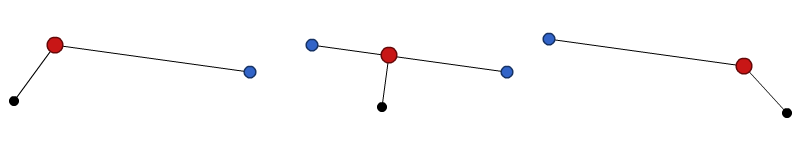
\includegraphics[width=0.9\linewidth]{../pictures/snap_points.png}
\caption{Snapping user point to border nodes (left,right) and snapping to perpendicular point where possible}
\label{fig:db_snap}
\end{figure}

With perpendicular projected point we create a \textit{new mock node} which represents the start point of our search on the road. We connect this new node with the end nodes of the closest segment, making it possible to use it in A* algorithm. We repeat the same steps for the end point. After the search we remove all the nodes and edges we additional added, reverting back the graph to the same state as before the search.

\subsection{Implementation in C++}
Road snapping function requires an extremely time consuming operation of finding close segments. One possible solution would be to actually calculate the perpendicular projections on every WaySegment in the database and then among them find the smallest. This would mean thousands of unnecessary calculations. Instead we used rtree data structure containing all the WaySegments implemented in \textit{Database class}. With this we were able to quickly find WaySegments whose bounding boxes intersect with our point. To compensate for areas, where roads are closely together, we implemented the search in small increasing steps. We start the with a small neighbourhood and gradually increase it, until we find any intersecting WaySegments. This approach reduces the calculations of perpendicular projections from thousand to just a couple. The diagram of the proces is shown in the figure \ref{fig:closestWaySegment}

\begin{figure}[h]
\centering
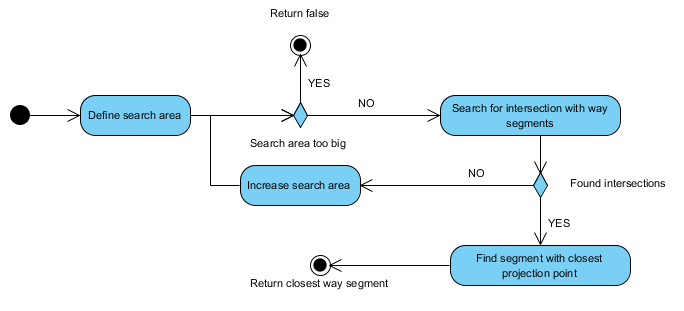
\includegraphics[width=0.7\linewidth]{../pictures/act_diagram_closest_way.png}
\caption{Diagram of finding the closest WaySegment}
\label{fig:closestWaySegment}
\end{figure}

\subsection{Implementation in Matlab}
Unfortunately Matlab does not have similar data structures capable of spatial filtering. To get the same end result we calculated the projection points on all the points and find the one with the minimal distance. To speed up the process of calculation we put the data in vectors and vectorize (\cite{matlab1}) the code for calculation. The speed of the calculation turned out to be sufficient.

\section{Shortest path A $->$ B}
This algorithm finds the shortest path between users defined points A and B on the roads that permit mode of transport selected by the user. With the usage of the road snapping functionality we can provide the user complete freedom in selecting the points anywhere on the map. The inputs to the algorithm are:
\begin{itemize}
\item Location of the start point
\item Location of the end point
\item Mode of transport
\end{itemize}
After finding the closest segments for start and end and adding mock nodes we can use A* algorithm to find the shortest path. The result of the algorithm is an object Path containing one PathSegment corresponding to WaySegments on the way from point A to B. If path does not exist we return an empty Path. The whole process is schematically shown on figure \ref{fig:ab_activity}.
\begin{figure}[h]
\centering
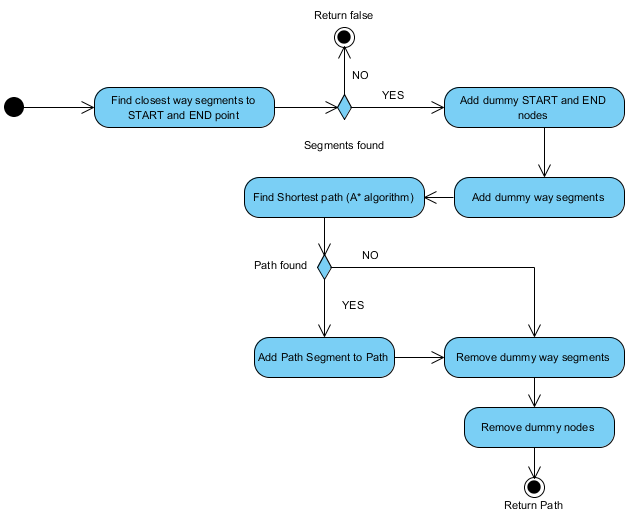
\includegraphics[width=0.8\linewidth]{../pictures/shortest_path_ab_activity.png}
\caption{Activity diagram of finding the shortest path between point A and B}
\label{fig:ab_activity}
\end{figure}

\subsection{Implementation}
The implementation details for both applications (C++ and Matlab) have been already described in specific methods of A* and road snapping. Other things are just sequence of if sentences that do not need special explanation.
Figures \ref{fig:ab_result_cpp} and \ref{fig:ab_result_matlab} shows the end result of the search as seen by the user.
\begin{figure}[h]
\centering
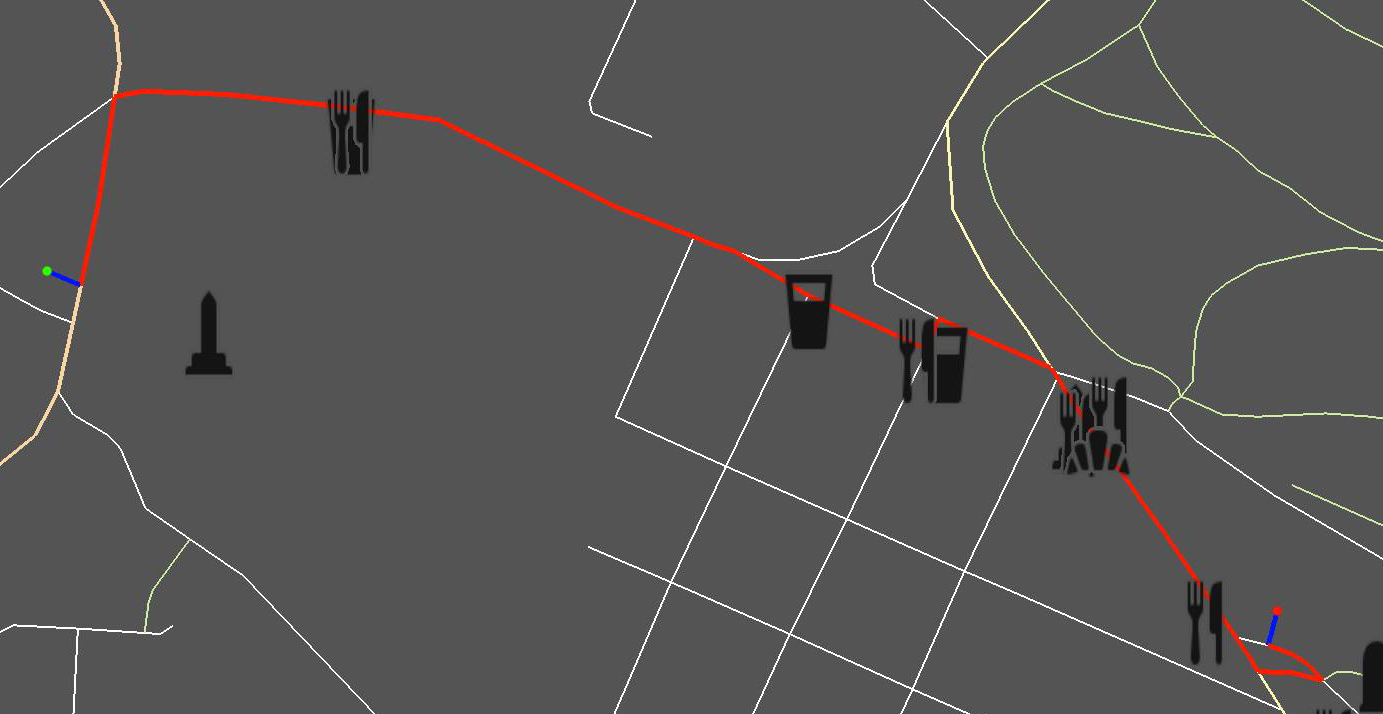
\includegraphics[width=0.8\linewidth]{../pictures/search_ab_result.jpg}
\caption{Result of the search for the shortest path as seen by the user in C++}
\label{fig:ab_result_cpp}
\end{figure}
\begin{figure}[h]
\centering
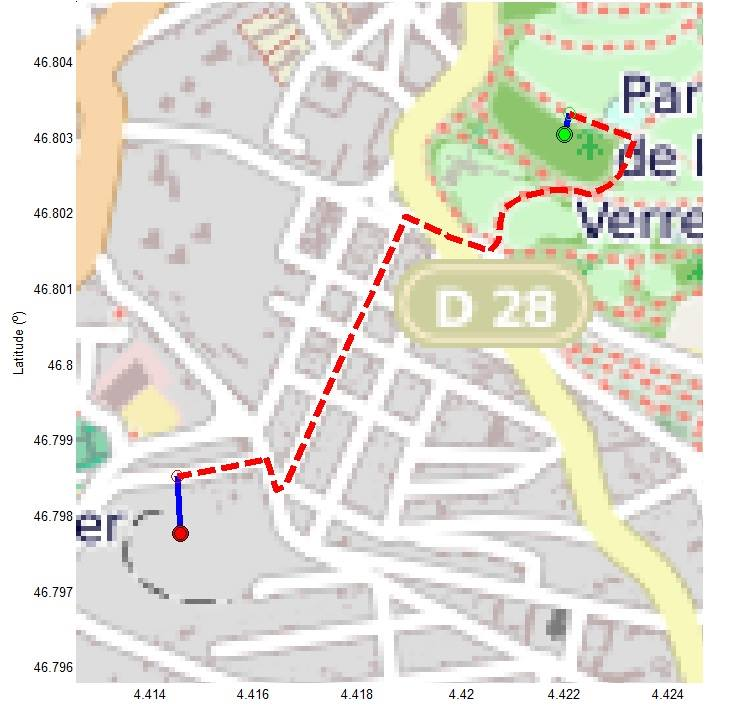
\includegraphics[width=0.6\linewidth]{../pictures/search_ab_matlab.jpg}
\caption{Result of the search for the shortest path as seen by the user in Matlab}
\label{fig:ab_result_matlab}
\end{figure}

\section{Radius search}
Radius search algorithm finds all the possible paths from user defined point A to all the points of interest (POIs) of a user specified category in some radius. The inputs to the algorithm are:
\begin{itemize}
\item Location of the start point
\item Category of POIs
\item Max distance of the path
\item Mode of transport
\end{itemize}
After finding the closest WaySegment to the start point, we go through all the POIs. For each of them we find the closest WaySegment and check the air distance between start and POI point. If the distance is bigger than the longest permitted path, we immediately discard the POI, because there is shorter way possible than that. Otherwise we try to find the shortest path using \textbf{Shortest path A $->$ B algorithm}. The final result of the algorithm is a bit different for both applications. In C++ we return the set of all possible paths ordered by the distance of the path, whereas in Matlab we only return the shortest path. Whole process is shown on figure \ref{fig:radius_activity}.    
 \begin{figure}[h]
 \centering
 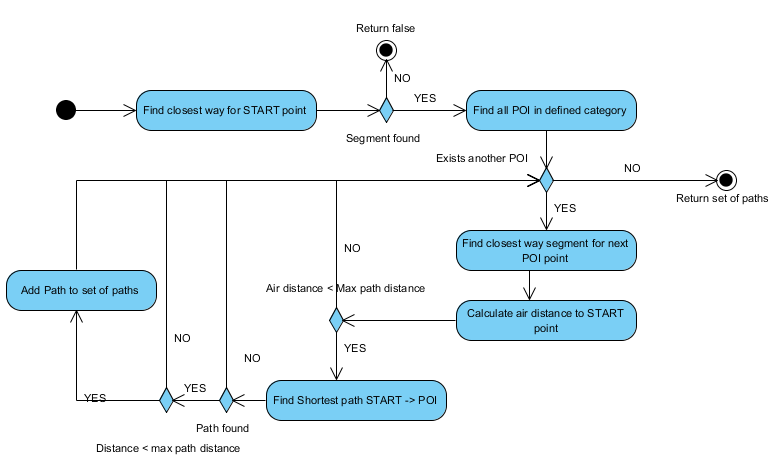
\includegraphics[width=0.8\linewidth]{../pictures/shortest_path_radius.png}
 \caption{Activity diagram of finding radius search between point A and POIs of specific categories}
 \label{fig:radius_activity}
 \end{figure}
 \subsection{Implementation in C++}
 As mentioned, data structure used to store all found paths is \textit{std::set}. We used that because our paths are unique and we want them ordered by distance. For this reason we implemented comparator that takes care of sorting the paths when they are inserted in the set. Figure \ref{fig:radius_result} shows the end result of the search as seen by the user.
 
\begin{figure}[h]
\centering
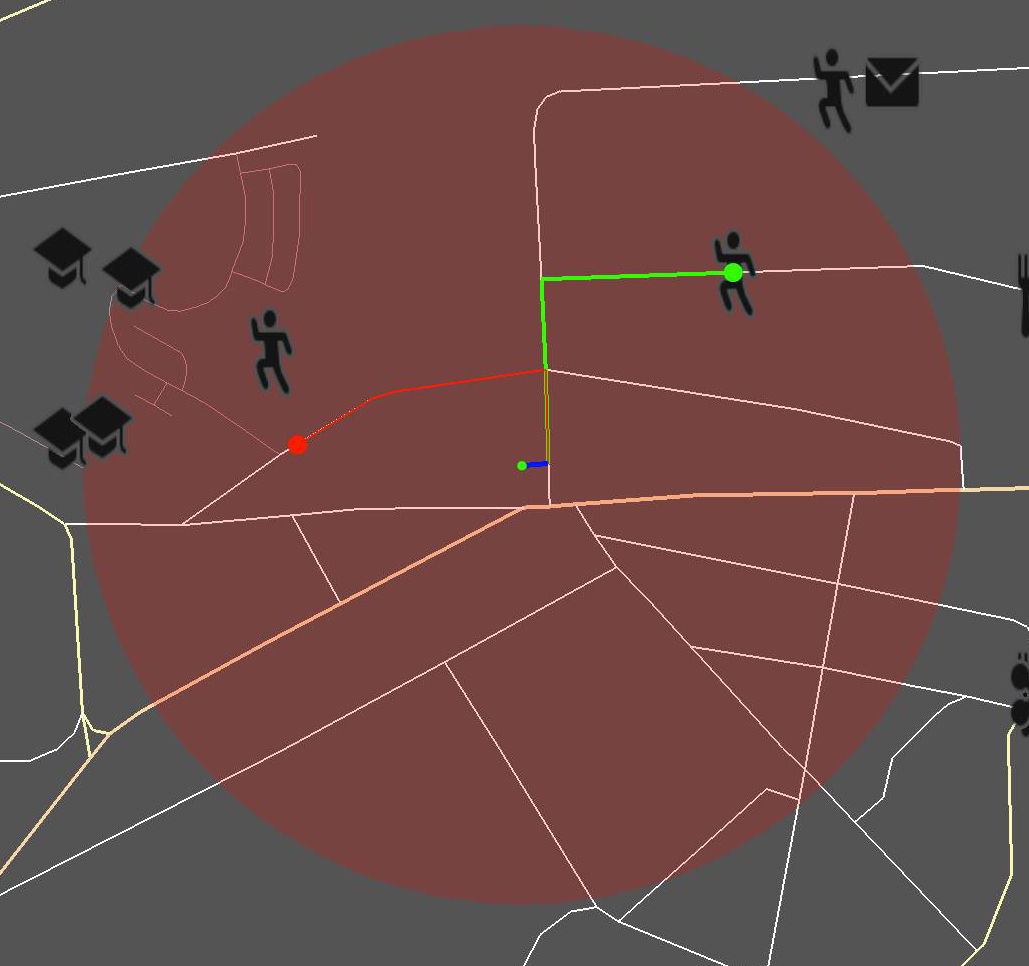
\includegraphics[width=0.8\linewidth]{../pictures/search_radius_result.jpg}
\caption{Result of the radius search as seen by the user in C++}
\label{fig:radius_result}
\end{figure}

 \subsection{Implementation in Matlab}
 In Matlab we implemented the algorithm using vectors and with the usage of vectorization. The calculations are not as efficient as in C++, but the usage of vectorization enables us to have results in sufficient amount of time. 
 
 
\section{Itinerary search}
Itinerary search algorithm constructs a path, that connects users defined start and end point and go through points of interested of a user defined categories. Algorithm finds a path that goes through one of the POI of each of the categories. The number of the categories in the list (points we want to visit) is not limited by the algorithm, but we have limited it in UI, because we have to be aware that the number of combinations increases significantly with every new category. Algorithm's inputs are:
\begin{itemize}
\item Location of the start point
\item Location of the end point
\item List of Categories of POIs we want to visit
\item Max distance of the path
\item Indication if the order of visited categories is important
\item Mode of transport
\end{itemize}
Before the start of actual path finding, we construct all possible combinations of POIs on the way. As already mentioned, for each category in the list we want to visit just one POI. We add list of points for each of the combinations to a queue which is ordered by ascending order of the sum of air distances of points on the path.
\par
Next phase is to find an actual path. We always look for the actual path of the list of points that have the smallest sum of air distance in the queue (top of the queue). If the air distance of the top element of the queue is bigger than the minimum distance found of the real path, we can stop the search, as we will not find smaller path then the one we already have. This way we do not keep looking for numerous paths which do not have any chance of being smaller, than the minimal path already found. Diagram in figure \ref{fig:itinerary_activity}] shows the process of the search. The same as in previous algorithms, if no path is found we return an empty path.
 \begin{figure}[h]
 \centering
 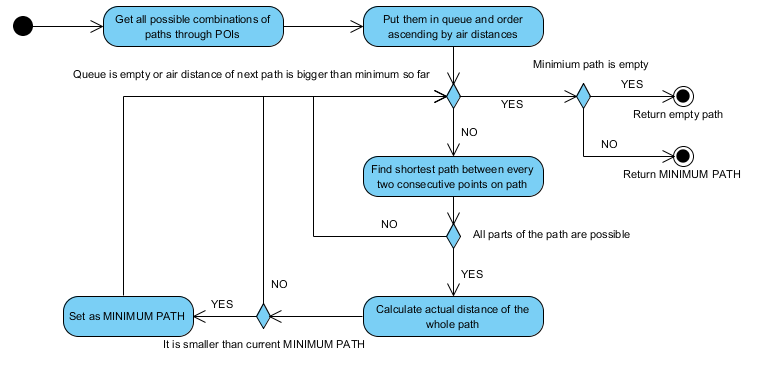
\includegraphics[width=0.7\linewidth]{../pictures/shortest_path_itinerary.png}
 \caption{Activity diagram of finding shortest path from A to B through POIs of specific categories}
 \label{fig:itinerary_activity}
 \end{figure}
 
\subsection{Implementation in C++}
Described algorithm was implemented in C++, using list data structure, to hold all the possible combinations of POIs and priority queue to sort the paths according the air distances. We used the selected data structures because they provided exactly what we needed. Priority queue because the order of our data is important and the smallest(largest) element goes out first. Figure \ref{fig:ite_result_cpp} shows the end result of the search as seen by the user.
\begin{figure}[h]
\centering
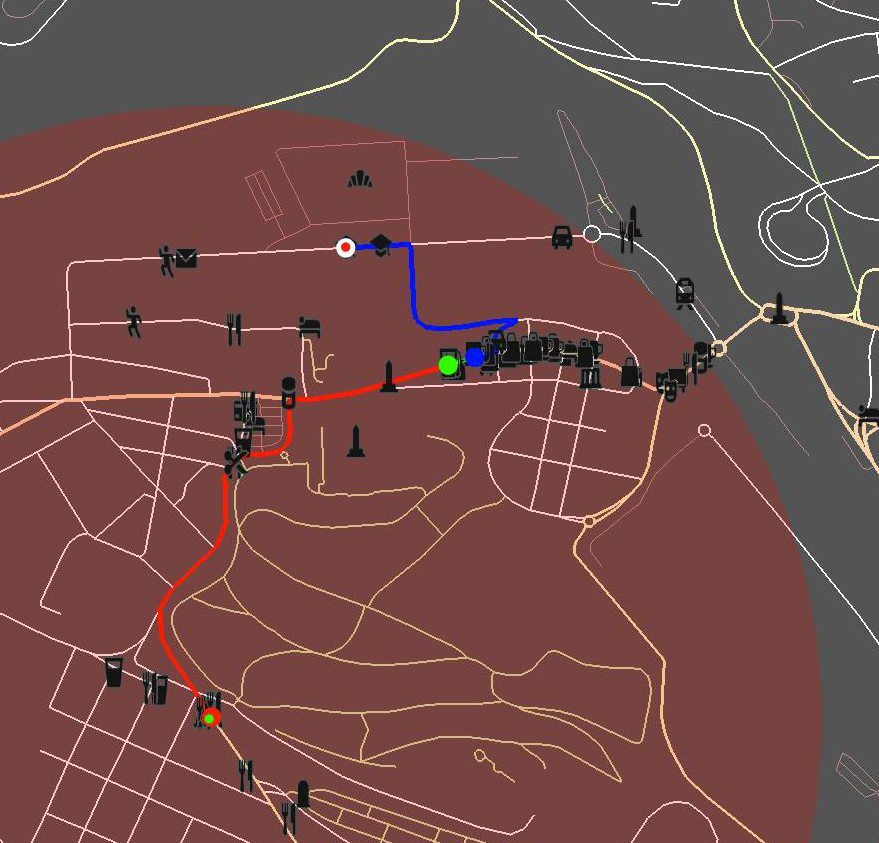
\includegraphics[width=0.8\linewidth]{../pictures/search_ite_result.jpg}
\caption{Result of the itinerary search as seen by the user in C++}
\label{fig:ite_result_cpp}
\end{figure}
\subsection{Implementation in Matlab}
In Matlab we have implemented the algorithm with only one middle category. In the calculations we take advantage of Vectorization, which significantly increases the speed of the calculations. Figure \ref{fig:ite_result_matlab} shows the end result of the search as seen by the user.   
\begin{figure}[h]
\centering
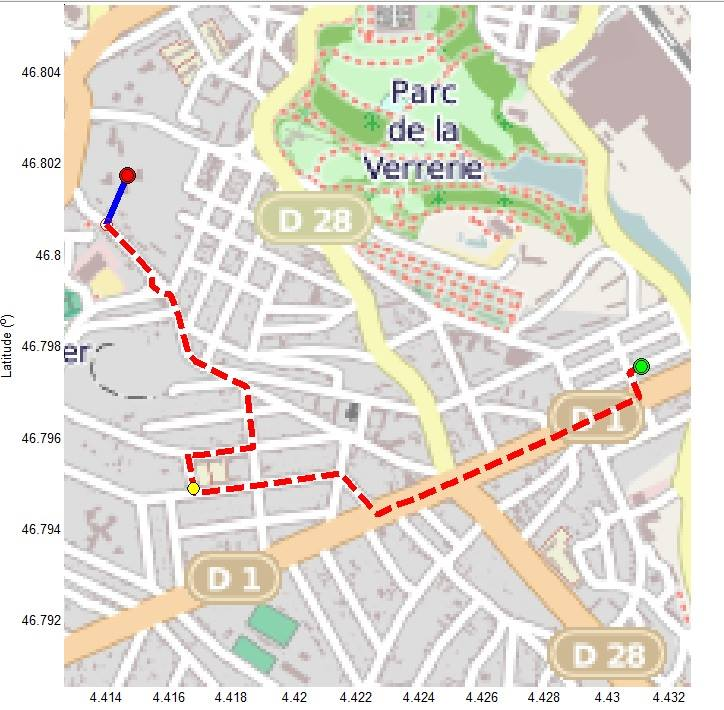
\includegraphics[width=0.6\linewidth]{../pictures/search_ite_matlab.jpg}
\caption{Result of the itinerary search as seen by the user in Matlab}
\label{fig:ite_result_matlab}
\end{figure} 
%\input{Chapters/Chapter7} 
% Chapter 8

\chapter{GUI} % Main chapter title

\label{Chapter8} % For referencing the chapter elsewhere, use \ref{Chapter1} 

\lhead{Chapter 8. \emph{GUI}} % This is for the header on each page - perhaps a shortened title

%----------------------------------------------------------------------------------------

\section{C++}
	C++ Part
\section{Matlab}
	Graphical user interface is main connection link between user and the program. By the correctly representation of data in GUI user can get all information that he needs. That is why it is so important to implement user interface that from the one hand will be easily understandable by user, and on the another hand can represent all possibilities of the program. In this chapter we will represent GUI for C++ and Matlab part, discuss its main features and difficulties.
	
	\subsection{MATLAB GUI}
	
		\subsubsection{Creating GUI with GUIDE Layout Editor}
			For creation GUI in MATLAB the GUIDE Layout Editor was used. It allows design graphically user interface and then generates code that corresponds to each element of the user interface. GUI can be consists of standard elements like axes, toggle buttons, push buttons, panels and others.\\
			
			Yomap MATLAB GUI is represented on figure 721 and consists from next elements:
			\begin{itemize}
				\item figure
				\item axes
				\item panels
				\item textboxes
				\item checkboxes
				\item toggle buttons
				\item push button
				\item static text
				\item pop-up menus
			\end{itemize}
			
			Here will be " Figure 721 – Yomap GUI representation in GUIDE Layout Editor". Natalia will provide.\\
			
			The final result of GUI is represented on figure 722 and has such functionality: 
			\begin{itemize}
				\item Zooming map in
				\item Zooming map out
				\item Pan map
				\item Plotting map layers
				\item Picking points on map with mouse click
				\item Choosing categories and points of interest by choosing from pop-up menu
				\item Choosing categories and points of interest with mouse click
				\item Enter name and address of the points of interest
				\item Enter coordinates of the points of interest
				\item Enable/disable middle point
				\item Hide/show search panel
				\item Show point of interest information
				\item Swapping points
				\item Choosing type of transport  
			\end{itemize}
			
			Here will be "Figure 722 - Yomap GUI"\\
			
			For zooming in, zooming out and pan map standard MATLAB functions were used. For others features callback functions were used. 
			User is allowed to enter name or coordinates of point of interest manually or with mouse click. In case of typing all information into textboxes it is verified and in case of error corresponding message is appear. If user prefers use mouse click coordinates are checking on being in range of the map.
			Another feature of the Yomap GUI is hiding/showing search panel (figure 723). Because sizes of the map are not allowed to show map and search panel together on the screens with small resolutions we decided to hide a panel for better map representation. In case if button “Hide All” is pressed the search panel became invisible and panel with instructions moves to the bottom of graphic window to show the whole map. After pressing button again all panels appear back on their initial places. 
			
			Here will be "Figure 723 – Yomap GUI search panel"
			
			For user convenience button “swap” was implemented (figure 724). In case of the same type of point of interest representation after pressing button “swap” all information between two points changes.  
			
			Here will be "Figure 724 – Yomap GUI “swap” button"
			
			All possible information about points and way is represented in instruction panel (figure 725). 
			
			Here will be "Figure 725 – Yomap GUI instruction panel"
			
		\subsubsection{Map Layers Plotting}
		Map by itself is complicated graphical structure that contains luck of information. That is why one of the biggest problems can appear in map representation is its overloading with information. So to prevent this and for user convenience we decide to use layers for plotting map. 
		Each layer represents only one type of information. In our GUI we have 4 main layers:
		\begin{itemize}
			\item Map Layer
			\item Roads Layer
			\item Way Layer
			\item Category Layer
		\end{itemize}
		
		Map layer (figure 726) is a *.png image of map of Le Creusot that loads in the beginning of the program. 
		
		Here will be "Figure 726 – Map layer"
		
		Roads layer (figure 727) is a vector of location of nodes that we traverse in order to have way from point A to point B.
		
		Here will be "Figure 727 – Roads layer"
		
		Way layer (figure 728) is a vector that shows the shortest way from point A to point B.
		
		Here will be "Figure 728 – Way layer"
		
		Category layer (figure 729) is a representation of points of interest on the map.
		
		Here will be "Figure 729 – Category layer"
		
		Each layer can be shown either by itself either in a combination with others layers. Because MATLAB allows draw any graphics on each other in a row the function "map\_Show\_Result" was implemented. Any time if one of the layers buttons is pressed the function is called and conditions of all layers buttons are sent to it. Before any layer appeared function "prepareMap" is called. It allows preparing axes before drawing layers and after this depending on buttons value corresponding layer is drawn. Way layer can be drawn only in case if route between point A and B is found.
		
		\subsubsection{Mouse Click And Dots Plotting}
		As was already mentioned user is allowed to pick any point on the map using mouse. To pick any point MATLAB functions "WindowButtonDownFcn" and "get(handles.mapDraw,'currentpoint')" are used. Result of these functions returns coordinates of the axes at the place where mouse button was pressed (figure 7210). 
		
		Here will be "Figure 7210 – Mouse click"
		
		In case if user chooses "show on map" as a point representation then he allows to take any point on the map even if “show category” button pressed. In case if "show category" button pressed but user choose "category search" or "search by enter" then he can pick only category points, otherwise point could not be plotting and data could not be saved. Any points that picked on the map are checked on being not out of range (figure 7211).
		
		Here will be "Figure 7211 – Out of range checking"
		
		Dots’ plotting after mouse click is the most difficult and "unstable" layer. The problem is in plotting dots for every point with saving map layers. We should always take into account how many points do we have, which of them are already plotted, which we need to plot and etc… 
		To solve this problem we used flag and handle to each point. Flag allows us to check if point already plotted or not and handle is used for deleting/plotting dot. For plotting dots function "draw\_point" was implemented. 
		To avoid problems with plotting points and layers algorithm that shown on figure 7212 was developed. It allows to draw any point on any layer independently.
		
		Here will be "Figure 7212 – Dots plotting algorithm"
 
% Chapter 8

\chapter{C++  vs MATLAB} % Main chapter title

\label{Chapter8} % For referencing the chapter elsewhere, use \ref{Chapter1} 

\lhead{Chapter 8. \emph{C++  vs MATLAB}} % This is for the header on each page - perhaps a shortened title

%----------------------------------------------------------------------------------------

\paragraph{}
	First of all the main difference between C++ and MATLAB is its cost. There are a lot of free and commercial implementations of C++ for different platforms. MATLAB on its term is only in charge. Of course student version of MATLAB exists, but it does not have some of toolboxes that can be very useful. 

\paragraph{}
	Beside this as we repeatedly noticed MATLAB has extremely high CPU and memory usage in comparison with C++. So it takes a lot of time for huge data calculation.

\paragraph{}
	From other point of view MATLAB is more flexible tool. Even if it takes more resources for data calculation representation of the data is more “free”. It is much easier to work with matrices, strings and other data in MATLAB than in C++. There is no need in variables declaration in MATLAB like in C++, we can use any variable in any part of program without caring of its type.

\paragraph{}
	Another MATLAB particularity is its global variables. In C++ global variable that declared in the beginning of the program became global for all program cycle. In MATLAB declared global variable is global only inside function. To use it in another function we need also declare it as a global in this function.

\paragraph{}
	One more difference between MATLAB and C++ is a huge amount of toolboxes in MATLAB. It allows to make different experiments without big effort. For example plotting graphs, made difficult calculations.

\paragraph{}
	Other difference is graphical user interface creation. C++ provides an extensive choice of methods and tools for GUI implementation. MATLAB in its turn has limited set of tools for this purpose, that does not give such big opportunities like in C++.

\paragraph{}
	Thus we can conclude that both C++ and MATALB are powerful tools, but must take into account that they should be chosen correctly depends on the existing problem.



%----------------------------------------------------------------------------------------
%	THESIS CONTENT - APPENDICES
%----------------------------------------------------------------------------------------

\addtocontents{toc}{\vspace{2em}} % Add a gap in the Contents, for aesthetics

\appendix % Cue to tell LaTeX that the following 'chapters' are Appendices

% Include the appendices of the thesis as separate files from the Appendices folder
% Uncomment the lines as you write the Appendices

% Appendix A

\chapter{Appendix Title Here} % Main appendix title

\label{AppendixA} % For referencing this appendix elsewhere, use \ref{AppendixA}

\lhead{Appendix A. \emph{Appendix Title Here}} % This is for the header on each page - perhaps a shortened title

Write your Appendix content here.
%\input{Appendices/AppendixB}
%\input{Appendices/AppendixC}

\addtocontents{toc}{\vspace{2em}} % Add a gap in the Contents, for aesthetics

\backmatter

%----------------------------------------------------------------------------------------
%	BIBLIOGRAPHY
%----------------------------------------------------------------------------------------

\label{Bibliography}

\lhead{\emph{Bibliography}} % Change the page header to say "Bibliography"

\bibliographystyle{unsrtnat} % Use the "unsrtnat" BibTeX style for formatting the Bibliography

\bibliography{Bibliography} % The references (bibliography) information are stored in the file named "Bibliography.bib"

\end{document}  